\documentclass[a4paper,english, 11pt]{report}
\usepackage[utf8]{inputenc}
\usepackage[T1]{fontenc}
\usepackage{uiomasterfp}
\usepackage{graphicx}
\usepackage{url}
\author{Joe Bayer}
\title{TCP PEP}
\subtitle{Extension of a TCP Performance Enhancing Proxy to
Support Non-interactive Applications}

\begin{document}
\uiomasterfp[program={Informatics: Programming and System Architecture}, supervisors={Michael Welzl\and Kristjon Ciko}]

\tableofcontents

\chapter{Intro}

\chapter{Background}

\section{TCP/IP}
(Get inspired by intro of tcp transport converter)
Perhaps the most well known internet transport protocol is the Transmission Control Protocol (TCP). It provides reliable and in order delivery of packets using acknowledgements and re-transmissions~\cite{Eddy_2022}. However, as the demands of the internet has changed, TCP has not. Even though TCP has changed with minor extensions over the years, such as increased initial windows or new options, the core ideas has stayed the same~\cite{rfc8803}. Concepts as the end-to-end argument still play a vital role in how TCP is used in the modern internet. Especially congestion control is suffering under the illusion that all logic should be placed on the endpoints, even if it spans multiple different domains (wireless / wired).\\

A networks topology and demands will vary a lot, especially between wired and wireless domains:
\begin{itemize}
  \item \textbf{Wireless Domain}: Fluctuating bandwidth, high error rate, blocking, radio signals.
  \item \textbf{Wired Domain}: Steady bandwidth, low error rate, high throughput, Ethernet / fiber.
\end{itemize}

\begin{figure}[h] % htbp stand for "here", "top", "bottom", "page"
	\centering
	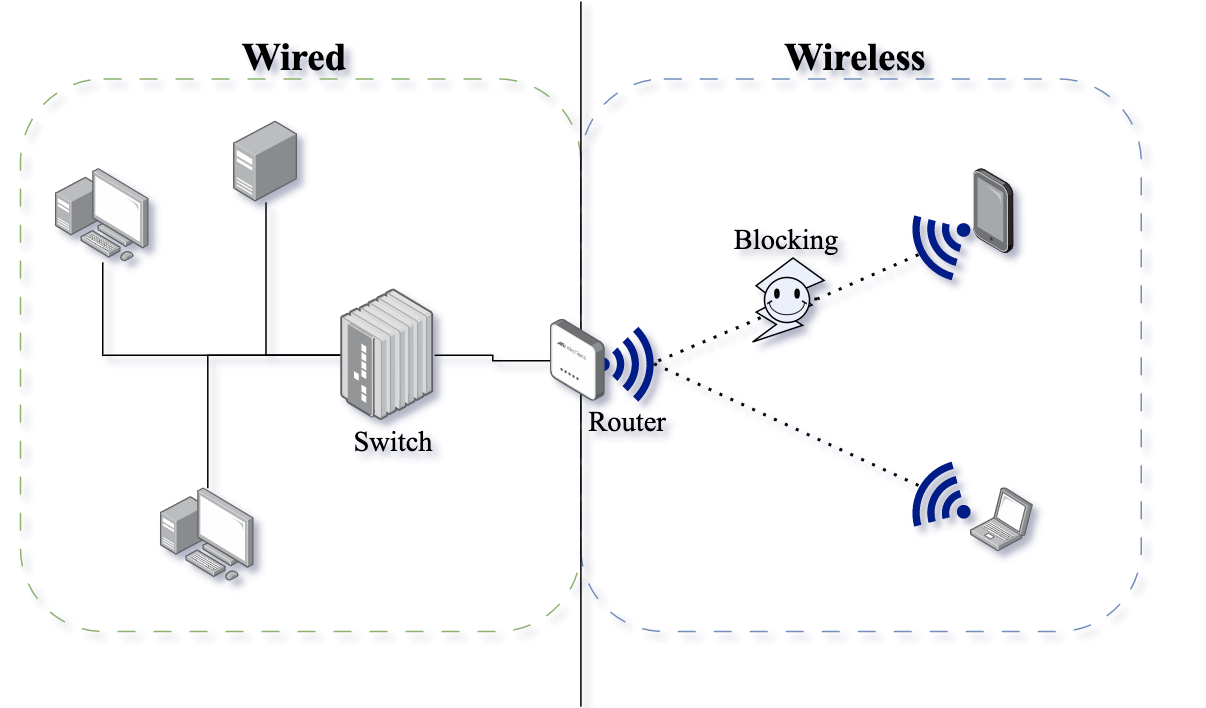
\includegraphics[scale=0.65]{../diagrams/drawio/domains.png}
  	\caption{5G bandwidth fluctuations from humans}
  	\label{fig:domains}
\end{figure}

Each domain has different requirements that a single TCP connection cannot provide. Fig. \ref{fig:domains} shows the two domains and their differences.

Interactive traffic uses TCP? {source}
End to end argument. Bad?
TCP handshake, reduce RTTs but using TCP Fast Open. Mostly short flows (cite)
\\
End to End congestion controller not very suited for highly fluctuating bandwidth.(cite David Hayes?)

.slow reactiveness of TCP~\cite{tcp_mmwave_proxy}.

\subsection{3 Way handshake (0 RTT)}
For TCP to establish a connection it uses a three-way handshake. First it sends a synchronization (SYN) packet to the desired endpoint. The endpoint answers with a acknowledgement and a synchronization packet of its own (SYN/ACK). And finally the client responds with a acknowledgment (ACK). At this point both endpoints have confirmed that they are ready for further communication. For any connection to be established this handshake has to be done. For short flows that terminate in just a few round trips the initial TCP handshake can be a bottleneck, which is made worse if the connection is using a proxy and has to exchange additional information. 

\subsection{Congestion Control}

\subsection{TCP Options}
A TCP connection can be configured with optional header extensions called TCP Options~\cite{tcp_options}.. 
Short flows terminating in a few round-trips. Meaning the "bottleneck" is the required initial TCP handshake.\\
TCP Fast Open allows data being exchanged during the handshake. 

Allow "syn fowarding" with TCP Fast Open creating a 0RTT increase when connecting through a proxy.
0RTT Transport Converter ~\cite{rfc8803}.


\section{Future of wireless communication.}
The future of wireless communication has seen a lot of improvements such as...
... highly increased bandwidth ... using Millimetre frequency bands ... but at the cost of Highly fluctuating bandwidth with wireless networks, especially with higher frequencies.\\ 

\subsection{5G Millimetre Wave}
The emergence of 5G Millimeter wave communications has opened the doors for low latency networks with multiple gigabit bandwidth. This is achieved by using higher millimetre wave (mmWave) frequencies in the range of 30GHz to 300GHz, which as a lot of benefits. ~\cite{Agrawal_Sharma_2016} A wider spectrum of frequencies to choose from and higher data transfer rates are just some of the many benefits mmWave provides. But along side the benefits, mmWave has also introduced a lot of new challenges.\\

A big problem with millimetre wave communication is signal path blocking also called "Line of sight blocking"~\cite{mmwave_blocking}. Its caused by the use of Beam-forming to increase the bandwidth and range of milimeter wave signals. Beam-forming focuses the signal in a certain direction making any blocking of the signal path devastating for the bandwidth. Even the human body can create enough blockage to drastically reduce the bandwidth. This causes huge fluctuations in the bandwidth whenever the signal is blocked. PICTURE?\\
\begin{figure} % htbp stand for "here", "top", "bottom", "page"
	\centering
	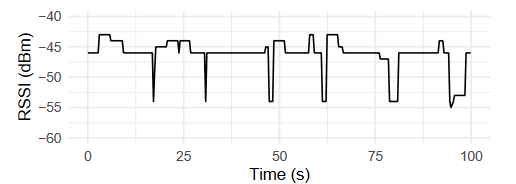
\includegraphics[scale=1.25]{../diagrams/graphs/tcp_mmwave_blockage.png}
  	\caption{5G bandwidth fluctuations from humans}
  	\label{fig:blockage}
\end{figure}

Fluctuating bandwidths lead to unstable TCP connections with a worst case of losing packets. Current TCP congestion controllers such as CUBIC, New Reno or New Vegas struggle when reacting to sudden fluctuating changes. They are simply not able to utilize the high bandwidth when it is available. Simply increasing the aggressiveness of a congestion controller is not a option either as it would disrupt the internet and not be TCP-friendly. A possible solution could be to buffer packets at the 5G (base) stations, having the data ready for when the bandwidth is high, this however creates a new problem bufferbloat.


\subsection{Buffering}
\subsubsection{Buffer bloat}
The buffer bloat problem occurs when the systems between the endpoints buffer so many packets that the latency drastically increases and the reliability of the network as a whole goes down.{https://lwn.net/Articles/507065/} The increased latency is detrimental for interactive (latency sensitive) applications. Generally its preferred to drop packets and keep buffers small to avoid buffering time sensitive packets such as synchronization packets. Although this works in most cases, its far from a optimal solution.\\\\

The increased bandwidth and low latency promises of new technology such as 5G has but a lot of pressure on the efficient forwarding of packets. Small buffers are therefore the standard, But at the same time, fluctuating bandwidth has shown the potential need to buffer packets for non-interactive traffic.

Most focus has been on (helping? Supporting?) latency sensitive applications like virtual reality or remote surgery to name a few. This thesis will explore non-interactive applications where latency is not that critical and more buffering is acceptable and most likely desirable. By splitting traffic into interactive and non-interactive we can improve the performance of both. By having very small buffers for interactive applications we avoid bufferbloat problems, while utilizing the benefits of big buffers for non-interactive applications.\\

\subsubsection{Packet Scheduling}
A method of reducing the effects off bufferbloat is packet scheduling. A system should not send more packets than the weakest link can handle {https://lwn.net/Articles/496509/}, this idea is built into TCP in the form of congestion control. However, when buffers grow to the point of causing bufferbloat, TCPs congestion control algorithms are unable to confidently determine a sending rate. Packet scheduling can solve this problem as it usually controls the size of the buffers. It makes sure queues can grow when needed, but keep the overall state of the buffers low. Packet scheduling has a lot more to offer than simple queue management, this will be explored later?

\subsection{Non-Interactive Applications}
Non-Interactive applications such as Web traffic, File transfers and Videos? can benefit from larger buffering, especially with fluctuating bandwidths. Being able to have packets buffered for when the bandwidth is high will decrease delay times. (need citation or prove it myself?). At the same time, interactive applications will not suffer under large queue delays.

\section{PEPs}
A performance enhancing proxy (PEP) is a (connection splitting) proxy designed to increase performance of applications using it. Already in use! (satelites, radio access networks, cite). Inherently increases performance?~\cite{tcp_mmwave_proxy}.
More logic inside the networks. Domain splitting and 0RTT.

\subsection{Transparent vs Non-Transparent}
A big discussion regarding PEPs has been if they should be transparent or non-transparent. Transparent PEPs are not visible to the applications that use it. They silently split the connections and spoof the IP-address of both the client and server~\cite{pep_dna}.. (SIDE EFFECTS). Non-Transparent PEPs on the other hand are explicitly chosen by either the client or the server, and the sender is aware of the proxy splitting the original connection. This approach can be seen as more ethical and "correct" (FIND BETTER WORDING), but modifications at the sender side become necessary to utilize the PEP.

\section{Kernel Modules}
LKM (Loadable Kernel Modules), "program" running inside the Linux kernel.
Userspace vs Kernel. Reduce system call overhead.
\subsection{System Calls}
Reduce over head from userspace -> kernel system calls.

\chapter{Implementation | Design}

{Table of design decisions based on different PEP implementations compared to ours.}
{0RTT, Transparent, Using TLV, Special ACKS, connection splitting.}\\
\begin{tabular}{ |p{4cm}||p{2cm}|p{2cm}|p{2cm}|p{2cm}| }
 \hline
 \multicolumn{5}{|c|}{PEP List} \\
 \hline
 Implementation& 0RTT &Connection Splitting &Special ACKs &Transparent\\
 \hline
 milliProxy   & AF    &AFG&   004 & x\\
 PEPDNA&   AX  & ALA   &248 & x\\
 SnoopTCP &AL & ALB&  008 & x\\
 Our PEP    &DZ & DZA&  012& x \\
 Transport Converter &   AS  & ASM&016& x\\
 ...& AD  & AND   &020& x\\
 ...& AO  & AGO&024& x\\
 \hline
\end{tabular}

\chapter{Evaluation}
\chapter{Conclusion}

\bibliography{myBib.bib}{}
\bibliographystyle{plain}
\end{document}s